% begin_generated_IBM_copyright_prolog                             %
%                                                                  %
% This is an automatically generated copyright prolog.             %
% After initializing,  DO NOT MODIFY OR MOVE                       %
% ================================================================ %
%                                                                  %
% (C) Copyright IBM Corp.  2011, 2011                              %
% Eclipse Public License (EPL)                                     %
%                                                                  %
% ================================================================ %
%                                                                  %
% end_generated_IBM_copyright_prolog                               %
\section {Third Generation Blue Gene (BG/Q)}

Highlights/Features:
\begin{itemize}
\item Resilient I/O framework providing higher availability for workloads.

\item Flexible workload architecture allowing not just single task (HTC) or entire block (HPC), but the 
full range of intermediate sizes including the ability to run multiple HPC (MPI) jobs on a single block.

\item Unification of multiple job submission models into an all-encompassing job submission command based 
on a client-multiplexer-server infrastructure.

\item Breaking the reliance of having an I/O node per block which is motivated by a higher ratio of compute 
nodes per I/O node. 

\end{itemize}

The latest supercomputer in the Blue Gene series is BG/Q which aims to reach multiple petaflops scaling 
when it is delivered. The archetypal BG/Q system called Sequoia will be installed at LLNL as a part of the 
Advanced Simulation and Computing Program. It will consist of 98,304 compute nodes comprising 1.6 million 
processor cores in 96 racks \cite{website:sequoia}.

\subsection{I/O resiliency}
\label{sec:io}
A significant change in the I/O architecture occurs with BG/Q and it brings significantly higher levels of 
resiliency and availability to Blue Gene workloads. Prior Blue Gene systems provided I/O nodes integrated on
the same board as compute nodes. For BG/Q the I/O nodes are now located on separate I/O drawers and I/O racks. 
With this hardware change, that at first appears to make the machine hardware less flexible, comes the 
opportunity to refactor the system software in a manner that actually makes it more flexible and resilient 
than the predecessor machines. This objective is achieved by BG/Q permitting hardware I/O resources to be 
booted independently of hardware compute resources. Previous Blue Gene generations would boot both the I/O
and compute resources present in a block and I/O issues could cause the entire block to fail causing any 
active jobs to be terminated. With BG/Q having the ability to mount file systems in a persistent manner, 
and not remounted every time a compute block is booted, comes the benefits of faster boot times and less 
start-up traffic to the file systems. In addition, new software functionality exists to allow for some 
degree of failing I/O nodes in an I/O block. When an I/O malfunction occurs the software will attempt to
re-route I/O traffic to other working I/O nodes and make efforts to recover the failed I/O nodes automatically. 
When successful the recovered nodes are placed back into service without any administrative involvement
and total transparency to running applications.  The only impact would be some degradation in overall
I/O performance for the application. This is very important when enabling many-task computing on 
Blue Gene. The added feature of I/O node 
failure resiliency means that all compute nodes remain active and eligible to run jobs, even in the 
face of a failure on an I/O node.  In the previous design on BG/P, the failure of an I/O node would 
render all connected compute nodes ineligible to run tasks.

\begin{figure}[!t]
    \centering
    \caption{BG/Q Job submission architecture.}
    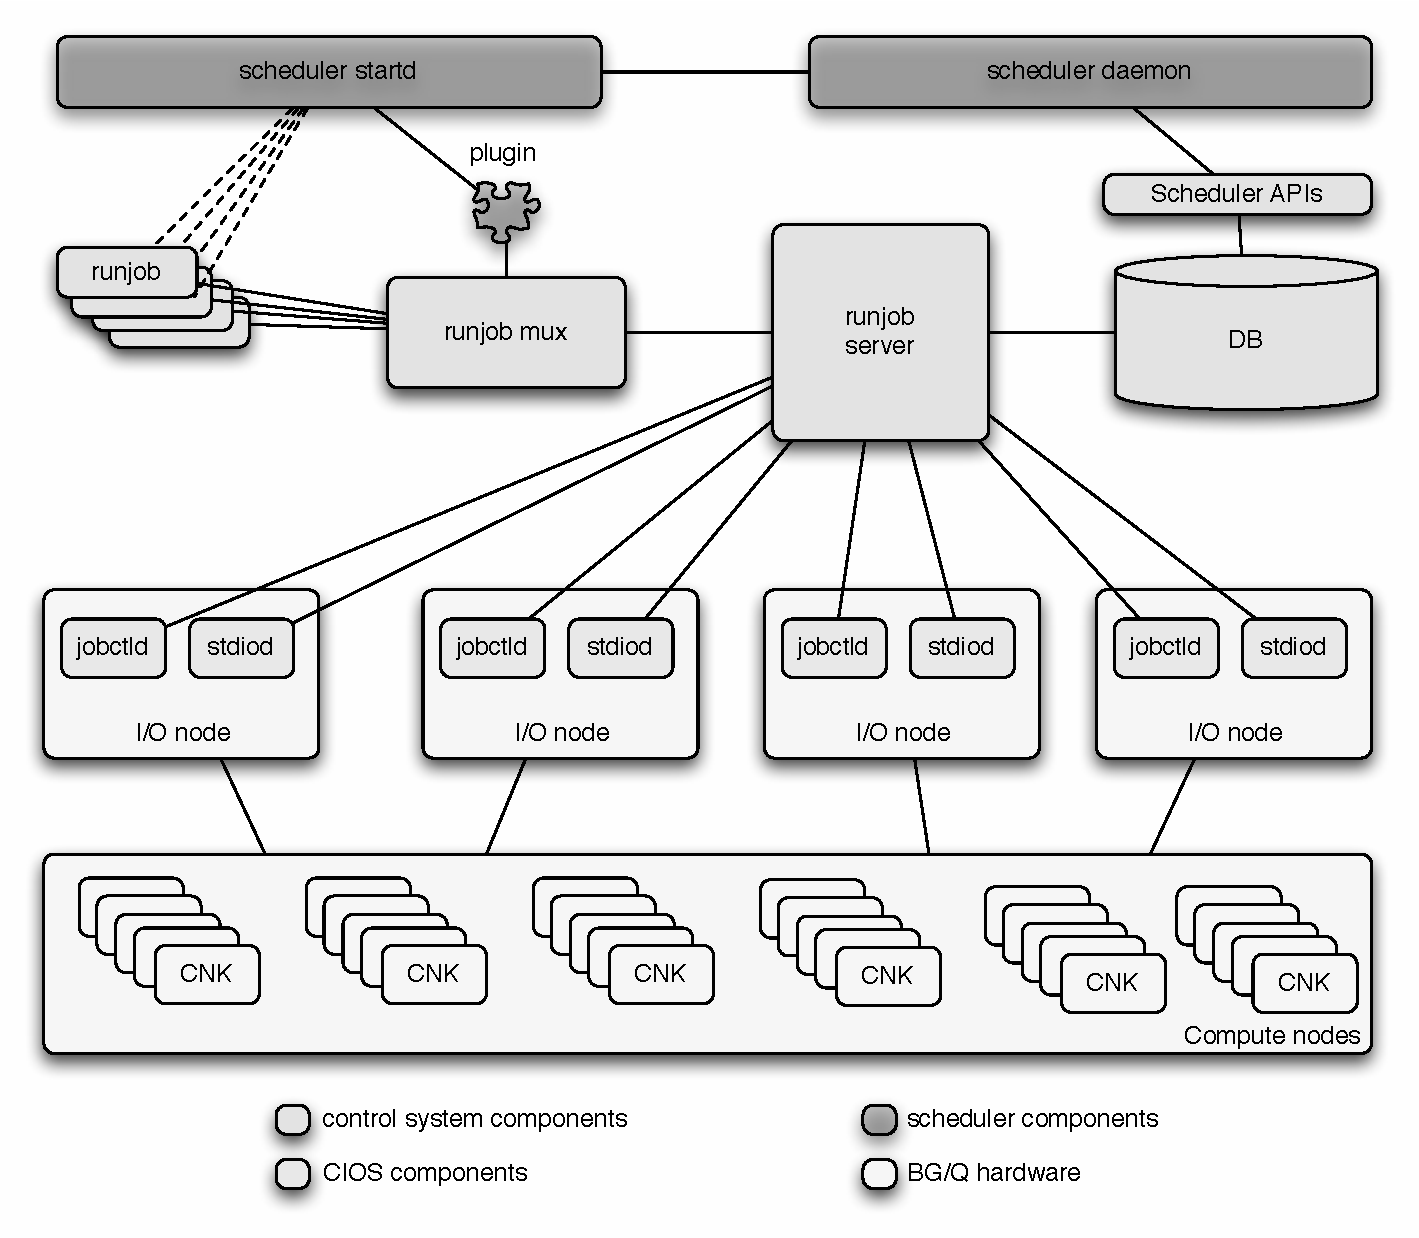
\includegraphics[width=3.5in]{jobsubmission}
    \label{fig:bgqjobsubmission}
\end{figure}

\subsection{Job Submission}
\label{sec:bgqjobsubmission}

The job submission architecture, shown in Figure \ref{fig:bgqjobsubmission}, has changed significantly 
when compared to the previous generation systems. It is somewhat based on the HTC job submission architecture 
shown in Figure \ref{fig:htcjobsubmission}. The most notable difference is the unification of HTC and HPC 
job submission components from BG/L and BG/P systems into a single consistent interface. The architecture 
also more closely resembles the HTC job submission architecture described in section \ref{sec:BGP} rather 
than the \emph{mpirun} or \emph{launcher} architecture described in section \ref{sec:BGL}.

Although the architecture is different, the objective and design goals of these job launch components are 
largely the same as previous designs. 

\begin{itemize}
\item{Fast and scalable job launch}
\item{Transparently relay standard output}
\item{Maintain state in a database}
\end{itemize}

\noindent
Three primary job submission components shown in Figure \ref{fig:bgqjobsubmission} help achieve these 
objectives. The \emph{runjob} component acts as a shadow of the job, its purpose is to parse arguments from 
the user or scheduler describing the job's resource requirements. Conceptually it performs the same actions 
as \emph{mpirun} or \emph{submit} from previous generation Blue Gene systems. Typically this component is 
executed under the user's credentials. The \emph{runjob\_mux} component acts as a traffic cop and gatekeeper. 
It obtains credentials from the \emph{runjob} component and performs some validation and sanity checking 
before forwarding the request to the \emph{runjob\_server}. The \emph{runjob\_server} component performs 
arbitration on the nodes each job has requested to use. This capability is significantly different than 
arbitration done by \emph{mpirun} due to the additional requirements imposed by sub-block jobs, which are 
described in section \ref{sec:subblockjobs}. The \emph{runjob\_server} also maintains job state in a database. 
Both the \emph{runjob\_mux} and \emph{runjob\_server} are executed under administrative credentials like 
the rest of the Control System.

\subsection{Compute Node Kernel}
\label{sec:cnk}
For BG/Q, job management in the CNK is more flexible compared to BG/P. As described in section \ref{sec:BGP}, 
a BG/P block is booted in a specific mode and CNK allocates and configures resources once.  There is no way to 
reconfigure resources without rebooting the block.  For BG/Q, the CNK allocates and configures resources with 
each job.  When a job is started, CNK is given information about the size and shape of the compute nodes 
participating in the job.  CNK uses that information to configure resources dynamically with each job.  
For example, a class route for the collective network that includes all of the nodes in the job is 
calculated with each job. This is equivalent to a MPI COMM\_WORLD communicator.  With I/O nodes located
on separate I/O blocks and CNK uses a service model for I/O instead of being hard-wired to a specific I/O node on 
the board.  This allows CNK to dynamically change which I/O node it uses for I/O services.

\subsection{Sub-block Jobs}
\label{sec:subblockjobs}

\begin{figure}[!b]
    \centering
    \caption{BG/Q Sub-block jobs.}
    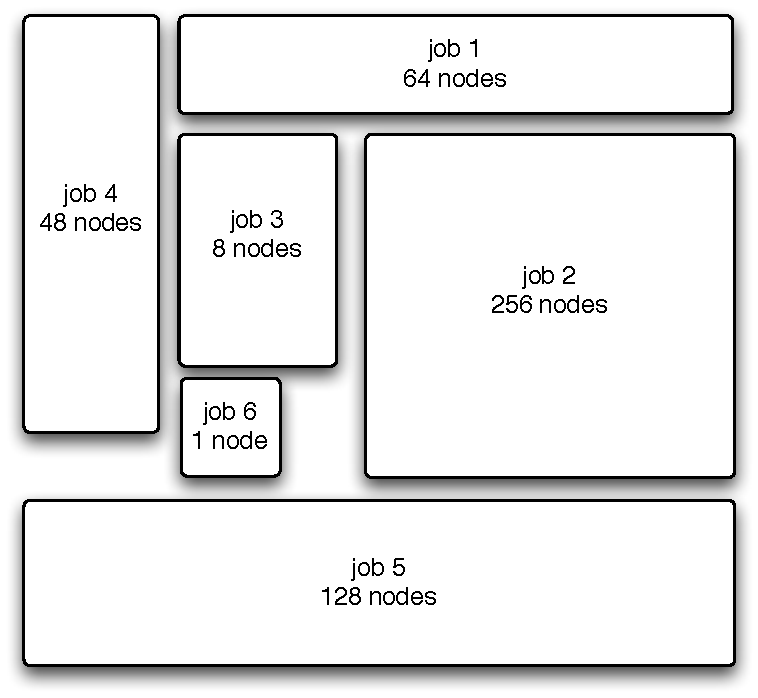
\includegraphics[width=3.5in]{subblockjobs}
    \label{fig:subblockjobs}
\end{figure}

While the concept of running multiple jobs on a single compute block was available on a BG/P system by
booting the block in HTC mode, it was limited to single node jobs without any ability to utilize the collective
networks between compute nodes. This concept is certainly useful for certain workloads, but the lack of a 
dedicated high speed communication network is severely limiting for many others. On previous Blue Gene systems,
messaging communication between multiple compute nodes within a job was only possible by using all of the compute nodes
in the entire block and idling the unused compute nodes should a job not need all them. This often led to 
significant fragmentation and under-utilization of the system when presented with a workload of thousands of 
jobs each needing a handful of compute nodes.

To address this problem, we describe a new software feature in BG/Q that we have termed \emph{sub-block jobs}.
This capability is enabled by the dynamic job configuration performed by CNK described in section \ref{sec:cnk},
and the physical separation of I/O and compute hardware described in section \ref{sec:io}. A sub-block job differs
from a job using the entire block by requesting a compute node corner location and five
dimensional shape at job launch time. This corner and shape are combined to logically create a sub-block, which
is then used for resource arbitration to ensure overlapping compute nodes are not in use by active jobs. It is 
also used to enforce the job is entirely contained within the corner compute node's midplane. Using a shape 
effectively enforces a collection of compute nodes without any holes, easing the challenges this would otherwise pose for the messaging 
communications software stack. The shape of a sub-block job has a maximum size of 512 compute nodes. This limitation is 
solely imposed by software and not due to a hardware limitation. The logic beind this restriction is a 512 node midplane is the 
building block for creating larger blocks. Doing so also greatly simplifies the resource arbitration. Any shape,
between a single node (1x1x1x1x1) and the entire midplane (4x4x4x4x2), is a valid shape for a sub-block job. Most
importantly, job sizes are not limited to a power of two, or by any artificial I/O ratio. 

Figure \ref{fig:subblockjobs} shows a two dimensional layout of six sub-block jobs using a variety of corner
and shape combinations. It is important to note the compute nodes in the empty space between the logical layout of the
jobs are available for use. They are not orphaned, reserved, or idled by another job.

There are several application considerations when using sub-block jobs. Foremost, the I/O resources are shared with other jobs 
serviced by the same I/O node. Considering the six jobs shown in Figure \ref{fig:subblockjobs}, one job could 
monopolize resources on the I/O node. If any of the five remaining jobs need guaranteed I/O bandwidth, 
precautions may need to be taken by the scheduler to ensure adequate resources are available. Secondly, sub-block jobs 
do not have the same electrical isolation guarantee that their full-block job counterparts do. On all Blue Gene systems, 
a block of compute nodes is electrically isolated from neighboring compute nodes when it is booted. Since sub-block jobs are 
sharing the same compute node to I/O node bridge, this guarantee cannot be enforced. This can be a security
concern to certain applications if they have a requirement to not share the torus links between compute nodes.

\subsection{Scalability}
\label{sec:scalability}
As described in section \ref{sec:bgqjobsubmission}, the job submission framework shown in Figure \ref{fig:bgqjobsubmission} 
is an enhanced extension of the HTC job submission architecture from BG/P shown in Figure \ref{fig:htcjobsubmission}. 
This is
\vfill\break
%spacing inplace to equalize column lengths on last page
%this must be done by hand

\noindent
in part due to the scaling strengths proven with that architecture. We anticipate 
this scalable design will be capable of handling workloads of tens of thousands of simultaneous jobs.
